\documentclass[12pt]{article}

% PAQUETES IMPORTADOS
\usepackage[utf8]{inputenc}                     %input encoding
\usepackage[a4paper, margin=2.5cm]{geometry}    %margins
\usepackage{sectsty}                            %tamanos de cabeceras
\usepackage[spanish,es-tabla]{babel}            %espanol
\usepackage{fontspec}                           %fuentes
\usepackage{anyfontsize}                        %tamanos de fuentes
\usepackage[style=ieee]{biblatex}               %bibliografia
\usepackage{csquotes}                           %citas a bibliografia
\usepackage{nameref}                            %referencia a capitulos
\usepackage{amsmath}                            %inline maths
\usepackage{amssymb}                            %math symbols
\usepackage{graphicx}                           %imagenes
\usepackage{color}                              %colores de fuentes
\usepackage{hyperref}                           %enlaces
\usepackage{ulem}                               %subrayados decentes
\usepackage{titlesec}                           %tamaños de títulos

% PROPIEDADES DE PAQUETES
\hypersetup{    % Color de enlaces (usados para referencias a capítulos)
    colorlinks,
    citecolor=black,
    filecolor=black,
    linkcolor=black,
    urlcolor=black
}

%tamaños de títulos
\titleformat*{\section}{\Huge\bfseries}
\titleformat*{\subsection}{\LARGE\bfseries}
\titleformat*{\subsubsection}{\large\bfseries}

% ARCHIVOS Y CARPETAS AUXILIARES
\graphicspath{ {./images/} }
\addbibresource{biblio.bib}

% FUENTES
\renewcommand{\contentsname}{Índice de Contenidos}
\setmainfont{Times New Roman}
\sectionfont{\fontsize{20pt}{15}\selectfont}
\subsectionfont{\fontsize{18pt}{15}\selectfont}
\subsubsectionfont{\fontsize{16pt}{15}\selectfont}

\begin{document}

%---------------------------------------------------
% PORTADA
%---------------------------------------------------
\begin{titlepage}
\begin{flushright}
\hfill\parbox[r][][c]{0.5\textwidth}{
{\fontsize{14}{14}\selectfont Universidad de Valladolid \\
E.T.S Ingeniería Informática \\
Grado en Ingeniería Informática\\
Rama de Ingeniería de Software\\
Cuarto Curso}}

\end{flushright}

\vfill
\centering
{\fontsize{16pt}{1cm}\selectfont \textbf{Resumen del Libro de la Asignatura <<Planificación y Gestión de Proyectos>>: Software Project Management}}


\vfill
\begin{flushright}
\hfill\parbox[r][][c]{0.4\textwidth}{
{\fontsize{14pt}{14cm}\selectfont
Bayón Sanz, Miguel
}
}
\end{flushright}

\end{titlepage}

%---------------------------------------------------
% INDICE
%---------------------------------------------------
\tableofcontents
\newpage

%---------------------------------------------------
% CUERPO
%---------------------------------------------------

%---------------------------------------------------
% Seccion 1
%---------------------------------------------------
\newpage
\section{Introducción a la gestión de proyectos Software}
\label{1.0.0}
\subsection{Introducción}
\label{1.1.0}

{Los proyectos de Software, al igual que otros proyectos, se basan en cumplir una serie de objetivos para satisfacer necesidades reales. Esto se hará encontrando a los inversores y sus objetivos. La gestión de proyectos tiene como finalidad cumplir sus objetivos, conociendo el estado del mismo proyecto en todo momento.}

\subsection[¿Por qué es importante la gestión de proyectos de Software?]{¿Por qué es importante la gestión de proyectos de Software?}
\label{1.2.0}

{Los proyectos de Software son el tipo de proyecto que más dinero mueve, implicando que una mala gestión haga que se pueda perder todo ese dinero. Según un estudio, de entre 13.522 proyectos:}

\begin{itemize}
    \item {El 66\% fracasa.}
    \item {El 82\% terminan tarde.}
    \item {El 43\% excede el presupuesto.}
\end{itemize}

\subsection{¿Qué es un proyecto?}
\label{1.3.0}

{Un proyecto es una \textbf{actividad planeada} que cuenta con la definición de todos los pasos y de su duración. Este cuenta también con una definición oficial establecida en el BSO ISO 10006 (1997): \textit{Proceso único consistente en un conjunto de actividades coordinadas y controladas con fechas de inicio y fin, promovido para conseguir un objetivo conforme a requisitos específicos incluyendo restricciones de tiempo, coste y recursos}.} \\

{El proyecto se encuentra en un término medio entre un trabajo rutinario y una investigación. Para diferenciarlos, debe cumplir los siguientes puntos:}

\begin{itemize}
    \item {Debe contener \textbf{tareas no rutinarias}.}
    \item {Requiere \textbf{planificación}.}
    \item {Debe cumplir \textbf{objetivos específicos}.}
    \item {Se debe completar en un \textbf{periodo de tiempo}.}
    \item {El trabajo se realiza \textbf{para otra persona}.}
    \item {Implica \textbf{varias especialidades}.}
    \item {Los empleados formarán un \textbf{grupo de trabajo temporal}.}
    \item {El trabajo se llevará a cabo en \textbf{varias fases}.}
    \item {Los \textbf{recursos} del proyecto estarán \textbf{limitados}.}
    \item {Debe ser un proyecto \textbf{grande y/o complejo}.}
\end{itemize}

{El tamaño del equipo es especialmente importante, porque implicará una mayor organización entre los participantes. Además, toda la experiencia ganada como equipo \textbf{se perderá al disolverse} el mismo (al ser grupos temporales).}

\subsection[Proyectos de Software vs otros tipos de proyectos]{Proyectos de Software vs otros tipos de \\proyectos}
\label{1.4.0}

{Algunas características de los proyectos de Software los hacen especialmente complicados:}

\begin{itemize}
    \item {\textbf{Invisibilidad}: el progreso no es inmediatamente visible.}
    \item {\textbf{Complejidad}: el proyecto de Software tiene gran complejidad por unidad monetaria.}
    \item {\textbf{Conformidad}: los desarrolladores se tienen que conformar con los requisitos de los clientes, que pueden ser cambiantes e inconsistentes.}
    \item {\textbf{Flexibilidad}: los sistemas Software están sujetos al cambio para acomodarse a elementos externos.}
\end{itemize}

\subsection[Gestión de contratos y gestión de proyectos técnicos]{Gestión de contratos y gestión de proyectos \\técnicos}
\label{1.5.0}

{En los proyectos internos se desarrolla para la misma organización. En los externos, al haber un contrato entre cliente y proveedor, existirán dos gestores de proyectos: uno del lado del cliente y otro del lado del proveedor. El del cliente (gestor del contrato) se ocupará de comprobar que el proyecto cumpla con los plazos y se ajuste al presupuesto, mientras que el del proveedor se ocupará de las decisiones de carácter técnico del proyecto.}

\subsection[Actividades cubiertas por la gestión de proyectos de Software]{Actividades cubiertas por la gestión de \\proyectos de Software}
\label{1.6.0}

{Un proyecto de Software suele pasar por \textbf{tres procesos} para generar un nuevo sistema:}

\begin{itemize}
    \item {\textbf{Estudio de viabilidad}: se evalúa lo que se quiere conseguir con sus requisitos y se comprueba que el proyecto sea viable. Si el proyecto es grande, el estudio de viabilidad puede ser un proyecto en sí mismo.}
    \item {\textbf{Planificación}: si el proceso anterior tiene un resultado positivo puede comenzar la planificación. Para proyectos muy grandes, la planificación no se detalla desde el principio, sino que se genera un guion general para todo el proyecto y se detalla solamente la primera etapa, dejando el resto para cuando se llegue a ellas.}
    \item {\textbf{Ejecución de proyecto}: El proyecto se ejecuta, a veces con sub-secciones de diseño e implementación. El libro, además, recalca la diferencia entre planificación (detallado de las actividades a llevar a cabo para generar un producto) y el diseño (decisiones sobre la forma del producto final).}
\end{itemize}

{Durante el proceso de implementación, surgirán actividades como las siguientes:}

\begin{itemize}
    \item {\textbf{Análisis de requisitos}: funciones o calidad mínima que serán requeridas por los usuarios del sistema.}
    \item {\textbf{Diseño de arquitectura}: Selección de los componentes (Software, Hardware o proceso de trabajo) que cumplirán cada requisito.}
    \item {\textbf{Diseño detallado}: Se diseñan independientemente las unidades que compondrán cada componente Software.}
    \item {\textbf{Programar y testear}: Escritura y depuración de cada unidad.}
    \item {\textbf{Integración}: Se prueban los componentes juntos.}
    \item {\textbf{Prueba de cualificación}: Se comprueba que todos los requisitos se cumplen.}
    \item {\textbf{Instalación}: El sistema trabaja en condiciones reales y/o para clientes.}
    \item {\textbf{Soporte de aceptación}: Resolución de errores en el sistema funcional. Una resolución de error puede ser un proyecto completo.}
\end{itemize}

\subsection{Planes, métodos y metodologías}
\label{1.7.0}

\begin{itemize}
    \item {\textbf{Metodología}: Conjunto de métodos.}
    \item {\textbf{Método}: Forma de trabajar o de organizar el trabajo.}
    \item {\textbf{Plan}: Organización de las tareas de un proyecto siguiendo una serie de métodos.}
\end{itemize}

\subsection{Algunas maneras de clasificar los proyectos de Software}
\label{1.8.0}

{Algunos factores a tener en cuenta al diseñar un proyecto son:}

\begin{itemize}
    \item {\textbf{Usuarios obligados contra usuarios voluntarios}: Un producto de uso empresarial contra un videojuego.}
    \item {\textbf{Sistemas de información contra sistemas embebidos}: Control de información contra control de máquinas.}
    \item {\textbf{Objetivos contra productos}: Solucionar un problema contra crear un nuevo sistema.}
\end{itemize}

\subsection{Stakeholders}
\label{1.9.0}

{Son aquellos que tienen un interés o una implicación directa en el proyecto o que se beneficiarán de él. Pueden ser:}

\begin{itemize}
    \item {Miembros del equipo del proyecto}
    \item {Externos al equipo del proyecto pero pertenecientes a la misma organización}
    \item {Externos a la empresa}
\end{itemize}

{Un buen líder de proyecto tiene que tratar de buscar los intereses de estos stakeholders y plasmarlos en el proyecto, buscando que todos obtengan beneficio de ello (La <<Theory W>> de Boehm and Ross, la situación \textit{win-win}).}

\subsection{Estableciendo objetivos}
\label{1.10.0}

{Algunos stakeholders serán los financiadores del proyecto y que además serán dueños del resultado y establecerán objetivos.}\\

{Los objetivos se definen como post-condiciones del proyecto que deben ser cumplidas para que el proyecto pueda tener éxito (por ejemplo, <<nuestro proyecto tendrá éxito si el cliente puede comprar productos online>>.}\\

{En caso de que varios stakeholders puedan tener derecho a la propiedad del proyecto, se establece una autoridad (generalmente un \textit{comité de dirección de proyecto}) con la potestad de establecer, vigilar y modificar objetivos. El líder de proyecto tendrá que reportarle los avances.}

\subsubsection{Sub-objetivos o metas}
\label{1.10.1}

{Al ser algunos objetivos muy generales (<<\textit{el proyecto será un éxito si reduce el consumo de energía}>>), se suelen dividir en sub-objetivos o metas fáciles de interpretar (<<\textit{para alcanzar este objetivo, será necesario...}>>).}\\

{Se suele definir un objetivo bien definido con el acrónimo \textbf{SMART}:}
\begin{itemize}
    \item {\textbf{S}pecific o específico: es concreto y está bien definido.}
    \item {\textbf{M}easurable o medible: debe ofrecer medidas (como \textit{reducir} o \textit{reducir en X unidad}) en lugar de conceptos abstractos (como \textit{mejorar}).}
    \item {\textbf{A}chievable o lograble.}
    \item {\textbf{R}elevant o relevante en cuanto al propósito del proyecto.}
    \item {\textbf{T}ime constrained o restringido en el tiempo: se tiene que poder completar en un tiempo determinado.}
\end{itemize}

\subsubsection{Medidas de efectividad}
\label{1.10.2}

{Las medidas de efectividad ofrecen una forma práctica de comprobar el cumplimiento de un objetivo.}

\subsection{Business case o Caso de negocio}
\label{1.11.0}

{El Business case forma parte del estudio de viabilidad y consiste en un análisis coste-beneficio y cuándo se conseguirá ese beneficio.}\\

{Los planes de proyecto deben asegurarse de que el Business case se mantiene intacto.}

\subsection{Éxito y fracaso de un proyecto}
\label{1.12.0}

{Un proyecto de Software suele ser un éxito si cumple:}

\begin{itemize}
    \item {Con la funcionalidad acordada.}
    \item {Con el nivel de calidad requerido.}
    \item {Que acaba a tiempo.}
    \item {Que acaba dentro del presupuesto acordado.}
\end{itemize}

{A veces, puede cumplir con estos términos pero no cumplir con el Business case (los beneficios superan los gastos). Esto significaría que el proyecto es un éxito pero es un fracaso empresarial, al igual que puede ocurrir que un proyecto sea un fracaso por romper varios puntos anteriores pero supere con creces el Business Case.}\\

{El Business Case busca presentar cuáles son los objetivos de negocio. Estos objetivos se pueden acercar a los objetivos de proyecto mediante actividades como evaluaciones de mercado o de usuarios.}\\

{Los proyectos, aun fracasando, pueden implicar adquisición de conocimientos o una mejor relación con el cliente que pueden llevar a que futuros proyectos puedan ser un éxito o puedan generar mejores ingresos.}

\subsection{¿Qué es la gestión?}
\label{1.13.0}

{Gestionar en un proyecto es:}

\begin{itemize}
    \item {Planificar tareas.}
    \item {Conseguir a los empleados adecuados.}
    \item {Dirigir.}
    \item {Controlar los progresos.}
    \item {Tomar medidas para remediar parones.}
    \item {Intervenir con los stakeholders.}
\end{itemize}

\subsection{Control de gestión}
\label{1.14.0}

{Cuando se prueban soluciones para resolver atascos en el proyecto, se debe monitorizar si estas soluciones dan o no resultado y buscar, en caso negativo, cuál es el verdadero problema del atasco. También se debe comprobar si la solución ha generado problemas paralelos al cambiar el plan inicial de proyecto.}

%---------------------------------------------------
% Seccion 2
%---------------------------------------------------
\newpage

\section[Evaluación de proyectos y gestión de programas]{Evaluación de proyectos y gestión de \\programas}
\label{2.0.0}
\subsection{Introducción}
\label{2.1.0}

{Además de las ganancias económicas directas, hay otras formas de decidir que un proyecto merece la pena. A veces, los beneficios de un proyecto producen ganancias indirectas y pueden combinar bien con el desarrollo de otros proyectos.}\\

{Este tema introducirá:}
\begin{itemize}
    \item {El desglose del \textbf{Business Case}.}
    \item {El \textbf{Programa de Proyectos}: conjunto de proyectos interrelacionados para la consecución de beneficios que no se obtendrían si se realizasen individualmente.}
    \item {El \textbf{Portfolio de Proyectos}: conjunto de programas y proyectos no necesariamente relacionados que se priorizan, seleccionan e implementan para lograr los objetivos estratégicos de la organización.}
\end{itemize}

\subsection{Un Business case}
\label{2.2.0}

{Un estudio de viabilidad, justificación de proyecto o Business case tiene como objetivo demostrar que los beneficios superarán los gastos. Suelen estar formados por los siguientes puntos:}

\begin{enumerate}
    \item {Introducción y antecedentes de la propuesta}
    \item {Proyecto propuesto}
    \item {Mercado}
    \item {Infraestructura organizacional y operacional}
    \item {Beneficios}
    \item {Esquema del plan de ejecución}
    \item {Costes}
    \item {Argumentos financieros}
    \item {Riesgos}
    \item {Plan de gestión}
\end{enumerate}

\subsubsection{Introducción y antecedentes de la propuesta}
\label{2.2.1}

{Describe un problema a ser resuelto o una oportunidad a ser explotada.}

\subsubsection{Proyecto propuesto}
\label{2.2.2}

{Breve esquema del proyecto.}

\subsubsection{Mercado}
\label{2.2.3}

{Necesario con nuevos productos. Describe la sección del mercado interesada y los posibles competidores.}

\subsubsection{Infraestructura organizacional y operacional}
\label{2.2.4}

{Describe cómo el proyecto cambiaría la estructura de la organización. Importante si implica modificar un sistema de información de una empresa.}

\subsubsection{Beneficios}
\label{2.2.5}

{Indica las ganancias o ahorros potenciales que generaría el resultado. Si el proyecto no pretende generar ganancias, convendría cuantificar el resultado.}

\subsubsection{Esquema del plan de ejecución}
\label{2.2.6}

{Contendrá un plan general del proyecto, además de otras decisiones como partes que se externalizarán a otras empresas, promoción o marketing, por ejemplo.}

\subsubsection{Costes}
\label{2.2.7}

{Se traduce el plan anterior en costes.}

\subsubsection{Argumentos financieros (\textit{financial case})}
\label{2.2.8}

{Se analizan los beneficios (en el momento del Business case será meramente especulativo). Esto se desarrolla en este tema.}

\subsubsection{Riesgos}
\label{2.2.9}

{Se analiza qué puede generar un fracaso en el proyecto (también especulativo). También se desarrolla en este tema.}

\subsection{Gestión del portfolio de proyectos}
\label{2.3.0}

{La gestión del portfolio de proyectos implica el reparto de recursos entre proyectos posibles y/o en desarrollo y comprobar qué proyectos merecen la pena y cuáles no para mantenerlos o abandonarlos, así como indicar las dependencias entre proyectos y asegurarse de no duplicar trabajo o no perder (u olvidarse de) trabajo necesario.}

\subsubsection{Definición del portfolio de proyectos}
\label{2.3.1}

{Se define qué proyectos van a estar en el portfolio, esto es, si van a estar todos los de la empresa o solo los que sean de cierto tipo: de nuevo producto, de actualización de producto, etc. Si todos los tipos de proyectos usan los mismos recursos, entonces se guardan todos en el mismo portfolio.}

\subsubsection{Gestión del portfolio de proyectos}
\label{2.3.2}

{Se indica en este mismo portfolio los costes detallados de los proyectos incluidos en él.}

\subsubsection{Optimización del portfolio de proyectos}
\label{2.3.3}

{Se monitoriza el rendimiento de los proyectos y se intenta compensar los proyectos que dan poco dinero pero son seguros con los que dan mucho pero tienen un riesgo alto.}

\subsubsection{Algunos problemas con la gestión del portfolio de proyectos}
\label{2.3.4}

{Puede haber problemas con los recursos que estén siendo usados en varios proyectos al mismo tiempo, ya que puede no estar apreciado el trabajo de estos en tareas rutinarias o en proyectos que sean tan pequeños que no se hayan mencionado en el portfolio.} \\

{Lo que se hace en estos casos es reservar un pequeño tiempo para los recursos en que pueden dedicarse a estas tareas no planeadas.}

\subsection{Evaluación de proyectos individuales}
\label{2.4.0}
\subsubsection{Evaluación técnica}
\label{2.4.1}

{Se comprueba si la funcionalidad puede ser conseguida con las tecnologías actualmente asequibles.}

\subsubsection{Análisis coste-beneficio}
\label{2.4.2}

{Se comprueba que un proyecto sea abordable dé o no beneficios. Para ello:}

\begin{itemize}
    \item {Se comprueban \textbf{todos} los costes y beneficios posibles y por haber de completar el proyecto.}
    \item {Se expresan estos costes y beneficios en la misma unidad monetaria.}
\end{itemize}

{La mayoría de costes se pueden agrupar en:}

\begin{itemize}
    \item {Costes de desarrollo y personal de desarrollo.}
    \item {Costes de implementación (puesta en marcha).}
    \item {Costes operacionales (post-puesta en marcha).}
\end{itemize}

\subsubsection{Previsión de cash flow}
\label{2.4.3}

{Muestra cuándo ocurrirán los gastos y beneficios. Típica y lógicamente, los gastos ocurrirán tiempo antes de los beneficios, que llegarán con el resultado final del proyecto. A esta previsión por lo general se le omite la inflación.}

\subsection{Técnicas de evaluación de coste-beneficio}
\label{2.5.0}

{A continuación se muestran las técnicas de evaluación con los ejemplos del libro. Se asume que los valores indicados son el total de todo el año ocurrido.}

\subsubsection{Beneficio neto}
\label{2.5.1}

{Se suma costes y beneficios de un proyecto totales. Este método tiene la ventaja de mostrar el beneficio final de un proyecto. Como desventaja se podría decir que no da importancia a cuándo se devuelve la inversión y que las estimaciones a largo plazo suelen ser muy inexactas.}

% Please add the following required packages to your document preamble:
% \usepackage{graphicx}
\begin{table}[ht]
\centering
\resizebox{\textwidth}{!}{%
\begin{tabular}{lllll}
Año            & Proyecto 1 & Proyecto 2 & Proyecto 3 & Proyecto 4 \\
0              & -100.000   & -1.000.000 & -100.000   & -120.000   \\
1              & 10.000     & 200.000    & 30.000     & 30.000     \\
2              & 10.000     & 200.000    & 30.000     & 30.000     \\
3              & 10.000     & 200.000    & 30.000     & 30.000     \\
4              & 20.000     & 200.000    & 30.000     & 30.000     \\
5              & 100.000    & 300.000    & 30.000     & 75.000     \\ \hline
Beneficio neto & 50.000     & 100.000    & 50.000     & 75.000    
\end{tabular}%
}
\caption{Beneficios Netos}
\label{tab:2.1}
\end{table}

\subsubsection{Periodo de recuperación de la inversión}
\label{2.5.2}

{Tiempo que tarda en igualarse el coste con el beneficio en un proyecto. Las empresas suelen escoger proyectos con menor periodo de amortización para reducir el tiempo en que están en deuda.} \\

{Como desventaja, ignora totalmente la rentabilidad del proyecto. Como ventaja, es sencillo y poco sensible a pequeños errores de previsión.}

\subsubsection{Retorno de inversión (ROI)}
\label{2.5.3}

{También Tasa de Rendimiento Contable (\textit{Accounting Rate of Return}, ARR), ofrece una medida de rentabilidad juntando ganancias, costes y tiempo. El porcentaje representa la media de beneficios en relación a la inversión por unidad de tiempo.}

\begin{equation}
    \text{ROI} = \frac{\text{average annual profit}}{\text{total investment}} \times 100
\end{equation} \\

{Por ejemplo, en el Proyecto 1 de la tabla~\nameref{tab:2.1}:}

\begin{equation}
    \text{ROI} = \frac{50.000/5}{100.000} \times 100 = 10\%
\end{equation} \\

{Lo que significaría que cada unidad de tiempo (año en este caso) se ganaría de media un 10\% de lo invertido.}

\subsubsection{Valor actual neto}
\label{2.5.4}

{El Valor Actual Neto (\textit{Net Present Value}, NPV) se entiende mejor por partes. El valor presente en un año concreto se calcula con esta fórmula:}

\begin{equation}
    \text{Valor presente} = \frac{\text{valor en el año t}}{(1+r)^t}
\end{equation} \\

{Donde $r$ es el interés aplicado (valor entre 0 y 1), $t$ es el número de años en el que se espera conseguir dicha ganancia y el valor en el año $t$ suele ser el beneficio neto predicho para ese año (ver \nameref{2.5.1}). El significado de esta fórmula se ve mejor de otra manera:}

\begin{equation}
    \text{Valor presente} \times (1 + r)^t = \text{valor en el año t}
\end{equation}

{Donde se ve claramente que, lo que estamos haciendo, es ingresar un dinero en una cuenta de ahorros (valor presente) con un interés concreto ($1 + r$) y durante $t$ años para conseguir el valor en el año $t$. Esta fórmula da importancia al momento del ingreso, siendo mejor cuanto antes llegue, por el beneficio potencial que pueda dar. Sin embargo, al estar calculando no el valor en el año $t$ sino el valor presente, lo que se hace es lo contrario: poner de manifiesto que, cuanto más tarde lleguen los ingresos, menos beneficios potenciales se generarán en las cuentas de ahorros.} \\

{En el libro, denomina \textbf{factor de descuento} al denominador de la fórmula original:}

\begin{equation}
    \text{Factor de descuento} = \frac{1}{(1+r)^t}
\end{equation} \\

{Finalmente, para sacar el Valor Actual Neto habría que sumar el valor presente de todos los años. Si aplicamos esto al Proyecto 1 de la tabla~\nameref{tab:2.1} con un interés del 10\% ($r = 0.1$):}

% Please add the following required packages to your document preamble:
% \usepackage{graphicx}
\begin{table}[ht]
\centering
\resizebox{\textwidth}{!}{%
\begin{tabular}{ccrl}
Año (t)                            & Cash-flow                     & \multicolumn{1}{c}{Factor de descuento} & \multicolumn{1}{c}{Valor presente} \\ \hline
0 & -100.000,00 & 1,0    & -100.000,00 \\
1 & 10.000,00   & 0,9091 & 9.091,00    \\
2 & 10.000,00   & 0,8264 & 8.264,00    \\
3 & 10.000,00   & 0,7513 & 7.513,00    \\
4 & 20.000,00   & 0,683  & 13.660,00   \\
5 & 100.000,00  & 0,6209 & 62.090,00   \\ \hline
\multicolumn{1}{r}{Beneficio neto} & \multicolumn{1}{l}{50.000,00} & NPV                                     & 618,00                            
\end{tabular}%
}
\caption{Valor Actual Neto}
\label{tab:2.2}
\end{table}

\newpage
\subsubsection{Tasa interna de retorno}
\label{2.5.5}

{La Tasa Interna de Retorno (\textit{Internal Rate of Return}, IRR) es una medida derivada del \nameref{2.5.4} en el que se busca calcular el interés $r$ que haga que el beneficio neto sea 0. Se usa sobre todo para comparar las rentabilidades de diferentes proyectos (cuanto mayor, mejor). El cálculo es complicado, se recomienda usar la función de Excel.}

\subsection{Evaluación de riesgos}
\label{2.6.0}

{Aquí se verán solamente los riesgos a nivel de negocio, no del proyecto.}

\subsubsection{Identificación y clasificación de riesgos}
\label{2.6.1}

{Se genera una matriz con cada riesgo y se evalúa su importancia y su probabilidad de ocurrir:}

\begin{table}[ht]
\centering
\begin{tabular}{lll}
Riesgo                                         & Importancia & Probabilidad \\ \hline
Pago online tiene problemas de seguridad       & M           & M            \\
Costes de mantenimiento mayores de lo esperado & L           & L            \\
Competidores recortan precios                  & H           & M            \\
...                                            &             &             
\end{tabular}
\caption{Ejemplo de matriz de riesgos}
\label{tab:2.3}
\end{table}

\subsubsection{Riesgo y valor actual neto}
\label{2.6.2}

{Cuando un proyecto es altamente arriesgado, se suele añadir un 2 o hasta un 5\% más de interés en el Valor Actual Neto.}

\subsection{Gestión de programas}
\label{2.7.0}

{Grupo de proyectos (que puede ser un subconjunto de un portfolio) que son gestionados de una forma coordenada para obtener beneficios que no hubieran sido posible obtener si se llevaran a cabo por separado.}

\subsubsection{Programas de ciclo de negocio}
\label{2.7.1}

{Colección de proyectos que coinciden en el año fiscal}

\subsubsection{Programas estratégicos}
\label{2.7.2}

{Proyectos que coinciden en área, meta, etc.}

\subsubsection{Programas de infraestructura}
\label{2.7.3}

{En empresas no dedicadas únicamente a TIC pero que tienen un departamento de informática, se agrupan los proyectos en programas de infraestructura.}

\subsubsection{Programas de investigación y desarrollo}
\label{2.7.4}

{Proyectos de I+D+i.}

\subsubsection{Asociaciones innovadoras}
\label{2.7.5}

{Conjunto de proyectos en los que se colabora con otra empresa.}

\subsection[Gestionando la asociación de recursos en programas]{Gestionando la asociación de recursos en \\programas}
\label{2.8.0}

{Un gestor de proyectos siempre tendrá que lidiar con el gestor de programas, que tendrá más autoridad a la hora de asignar recursos a proyectos:}

\begin{table}[ht]
\centering
\begin{tabular}{c|c}
Gestor de programas                                                    & Gestor de proyectos                                                       \\ \hline
\begin{tabular}[c]{@{}c@{}}Muchos proyectos\\ simultáneos\end{tabular} & \begin{tabular}[c]{@{}c@{}}Un proyecto a\\ la vez\end{tabular}            \\
\begin{tabular}[c]{@{}c@{}}Relación personal con\\ recursos habilidosos\end{tabular} & \begin{tabular}[c]{@{}c@{}}Relación impersonal\\ con los recursos\end{tabular}  \\
\begin{tabular}[c]{@{}c@{}}Optimiza el uso de\\ recursos\end{tabular}  & \begin{tabular}[c]{@{}c@{}}Minimiza la demanda\\ de recursos\end{tabular} \\
\begin{tabular}[c]{@{}c@{}}Suele ver los\\ proyectos como\\ similares\end{tabular}   & \begin{tabular}[c]{@{}c@{}}Suele ver los\\ proyectos como\\ únicos\end{tabular}
\end{tabular}
\caption{Gestor de Programas contra Gestor de Proyectos}
\label{tab:2.4}
\end{table}


%---------------------------------------------------
% Seccion 3
%---------------------------------------------------
\newpage
\section[Una revisión a la planificación de proyectos]{Una revisión a la planificación de \\proyectos}
\label{3.0.0}

\subsection{Introducción a la planificación de proyectos Step Wise}

{Step Wise son los pasos básicos a seguir en la planificación de un proyecto.}

\begin{figure} [ht]
    \centering
    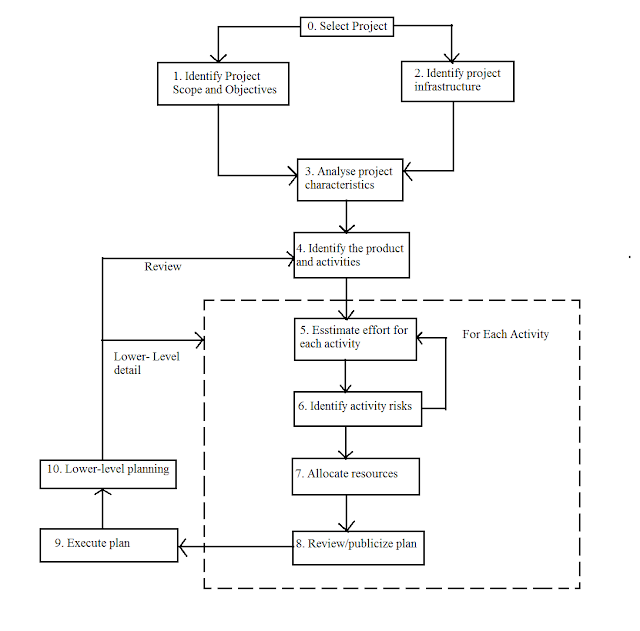
\includegraphics[width=\textwidth]{step_wise.png}
    \caption{Step Wise}
    \label{fig:3.1}
\end{figure}


%---------------------------------------------------
% BIBLIOGRAFIA
%---------------------------------------------------

\newpage
\section{Única bibliografía}
\nocite{*}
\begingroup
\renewcommand{\section}[2]{}%
\printbibliography
\endgroup


\end{document}